\documentclass[aps,nofootinbib,onecolumn,groupedaddress,a4paper]{revtex4}

\usepackage{color}
\usepackage{graphicx}
\usepackage[utf8]{inputenc}

\usepackage{listings}

\lstset{
  language=Python,
  showstringspaces=false,
  formfeed=\newpage,
  tabsize=4,
  commentstyle=\itshape,
  basicstyle=\ttfamily,
  morekeywords={models, lambda, forms}
}


\begin{document}

\title{Charge to Mass Ratio of the Electron} 

\author{Adnan Basar}
\affiliation{Phys 442.01\\
2010205108}


\date{March 15, 2013}

\begin{abstract}
This experiment uses the study of the motion of an electron that moves perpendicular to a magnetic field and measures the charge-to-mass ratio of electron.
\end{abstract}

\maketitle


\section{Introduction}


The charge to mass ratio of an electron is measured from observing the trajectories of electrons in a magnetic field. When  an electron moves in an electrostatic field from point 1 to point 2 with electric potential  difference V between them,  the electron will gain a kinetic energy (K) given by
\begin{center}
$K=\frac{mu^{2}}{2}=eV $
\end{center}
where	 e = charge  of the electron, m = mass of the electron, u = velocity of the electron. \\



When a charged particle of charge q with velocity u moves through a magnetic field  with magnetic field strength B,  it experiences a force ("Lorentz force") given by
\begin{center}
	$F = q(u x B)$
\end{center}

                                  

If B is perpendicular to u then the electron will move in a circle whose plane is also perpendicular to B, and the  magnetic force (Lorentz force) provides  the centripetal force for this circular motion, i.e.
\begin{center}
$\frac{mu^{2}}{r} = euB$
\end{center}
                             

where	 m = mass of electron
 r = radius of circular path.\\

Solve Eq. (3) for u and substitute into Eq. (1) to obtain an expression for the charge-to-mass ratio of the electron
\begin{center}
$\frac{e}{m}=\frac{2V}{(Br)^{2}}$
\end{center}

So if we know the magnitude of the magnetic field, the potential difference V and
the radius of the path r, we can calculate the charge-to-mass ratio of the
electron. For electrons (or any given kind of particle) the left hand side is a constant. For example, if we raise the energy of the electrons injected into  the magnetic field region (by increasing the accelerating potential V) , and we desire to maintain an orbit with the same radius, then this equation informs us we
would have to increase the magnitude of the magnetic field. Alternatively, if
we want to increase the radius of the circular orbit we would have to decrease
the magnitude of the magnetic field. The experimental problem is to generate a uniform magnetic field.\\

The setup consists of a fine beam tube and a pair of Helmholtz coils to produce the magnetic field. The field strength will be determined using the expression
\begin{center}

$B=\frac { 8{ \mu  }_{ o }IN }{ \sqrt { 125 } { r }_{ c } } $

\end{center}

where ${\mu}_{0}=1.257x10^{-6}$, $N=130$ turns and ${r}_{c}=15$ cm.\\



The experiment involves injecting electrons into a magnetic field generated by Helmholtz coils, which provide an approximately uniform magnetic field close to the center, but there is some non-uniformity which may affect the measurement.


\section{Experimental Setup}
In this experiment, the following apparatus are used:
\begin{itemize}
\item Fine Beam Tube Set (including the Helmholtz coils)
\item DC Power Supply (0-300 V)
\item Filament Power Supply (6.3 V AC, 5 A)
\item AC Ammeter (0-3 A)
\item DC Power Supply (0-5 A)
\item DC Ammeter (0-5 A)
\item DC Voltmeter (0-300 V)
\item Connecting Leads
\end{itemize}


\section{Data and Analysis}
For analysis part, there are some experimental data for both fixed voltage and magnetic field. And our known errors are ${\sigma}_{V}=10V$,  ${\sigma}_{r}=0.4cm$ and ${\sigma}_{I}=0.1A$  
\begin{table}[htdp]
\caption{ Experimental Data for fixed magnetic field $B$ at ($1A$)}
\label{rawdata}
\centering
\begin{tabular}{ccc}
\\
Voltage ($V$)  & $r$ (cm)  \\
\hline
110 &  3.8   \\
140 &  4.5   \\
180 &  5.1   \\
220 &  6.2   \\
280 &  7.0   
\end{tabular}
\label{default}
\end{table}%

With the values of Table I, we obtained Figure I by using the straight line fit to $y=mx+n$. The slope $m$ is $\frac{V}{{r}^{2}}$.Thus, $\frac{e}{m}=\frac{2m}{{B}^{2}}$. By using error propagation, we will obtain:

\begin{center}

${ { \sigma  }_{ \frac { e }{ m }  } }^{ 2 }={ \left( \frac { \partial  }{ \partial m } \left( \frac { 2m }{ { B }^{ 2 } }  \right)  \right)  }^{ 2 }{ { \sigma  }_{ m } }^{ 2 }\quad +\quad { \left( \frac { \partial  }{ \partial B } \left( \frac { 2m }{ { B }^{ 2 } }  \right)  \right)  }^{ 2 }{ { \sigma  }_{ B } }^{ 2 }={ \left( \frac { 2m }{ { B }^{ 2 } }  \right)  }^{ 2 }{ { \sigma  }_{ m } }^{ 2 }+{ \left( \frac { 2m }{ { B }^{ 2 } }  \right)  }^{ 2 }{ { \sigma  }_{ m } }^{ 2 }={ \left( \frac { -4m }{ { B }^{ 3 } }  \right)  }^{ 2 }{ { \sigma  }_{ B } }^{ 2 }$

\end{center}


\begin{figure}[h]
\caption{ Voltage vs. ${r}^{2}$  \label{rawplot}}
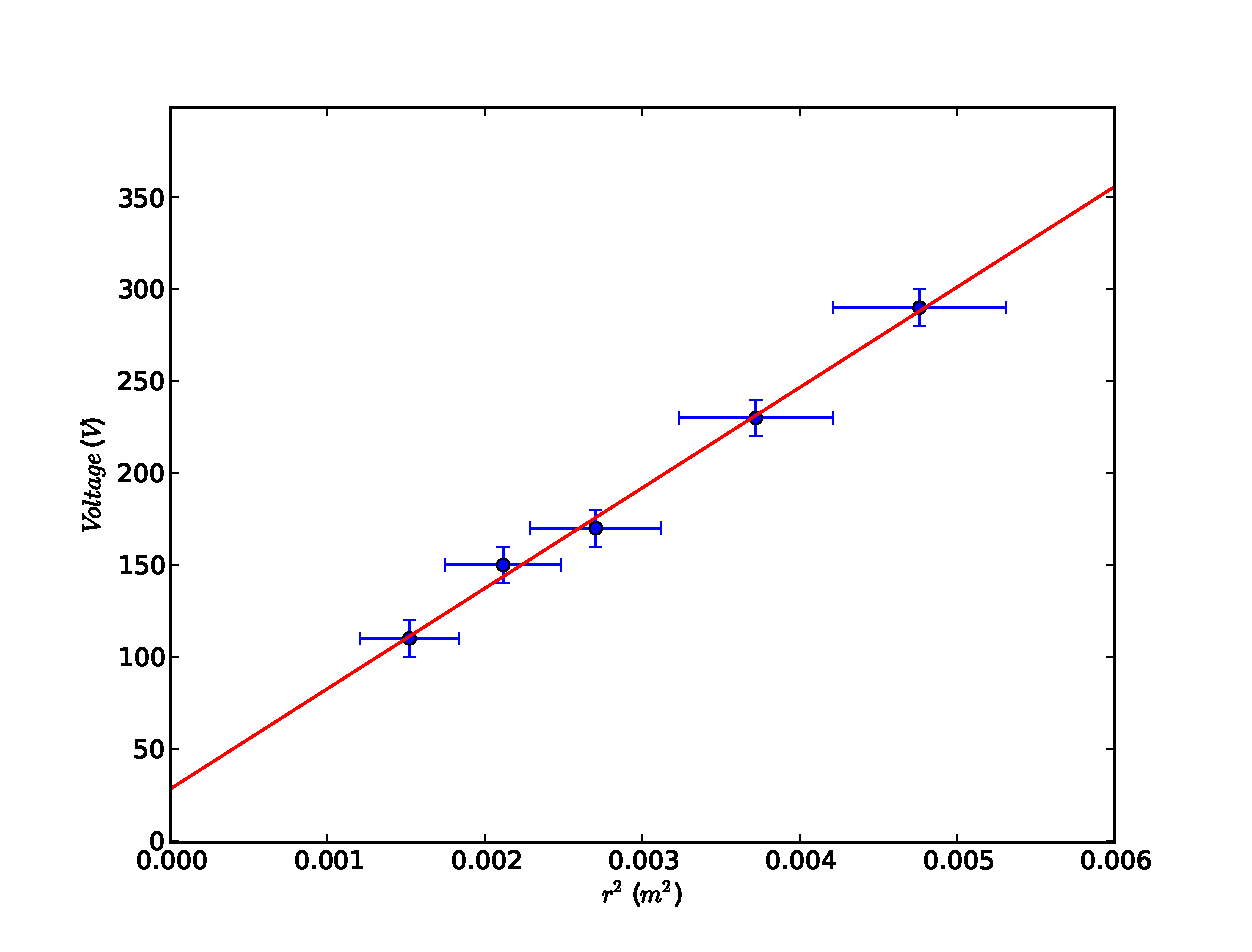
\includegraphics[width=0.5 \columnwidth]{fixedb.eps}
\end{figure}


\begin{table}[htdp]
\caption{ Experimental Data for voltage $V$ at ($250V$)}
\label{rawdata}
\centering
\begin{tabular}{ccc}
\\
Current ($A$)  & $r$ (cm)  \\
\hline
0.9 &  8.2   \\
1.3 &  5.3   \\
1.8 &  3.5   \\
2.2 &  3.3   \\
2.6 &  2.9   
\end{tabular}
\label{default}
\end{table}%

With the values of Table II, we obtained Figure I by using the straight line fit to $y=mx+n$. The slope $m$ is $\frac{1}{{Br}^{2}}$.Thus, $\frac{e}{m}=2mV$. By using error propagation, we will obtain:

\begin{center}

${ { \sigma  }_{ \frac { e }{ m }  } }^{ 2 }={ \left( \frac { \partial  }{ \partial m } \left( 2mV \right)  \right)  }^{ 2 }{ { \sigma  }_{ m } }^{ 2 }\quad +\quad { \left( \frac { \partial  }{ \partial V } \left( 2mV \right)  \right)  }^{ 2 }{ { \sigma  }_{ V } }^{ 2 }={ \left( 2V \right)  }^{ 2 }{ { \sigma  }_{ m } }^{ 2 }+{ \left( 2m \right)  }^{ 2 }{ { \sigma  }_{ B } }^{ 2 }$

\end{center}


\begin{figure}[h]
\caption{$1/{r}^{2}$ vs ${B}^{2}$  \label{rawplot}}
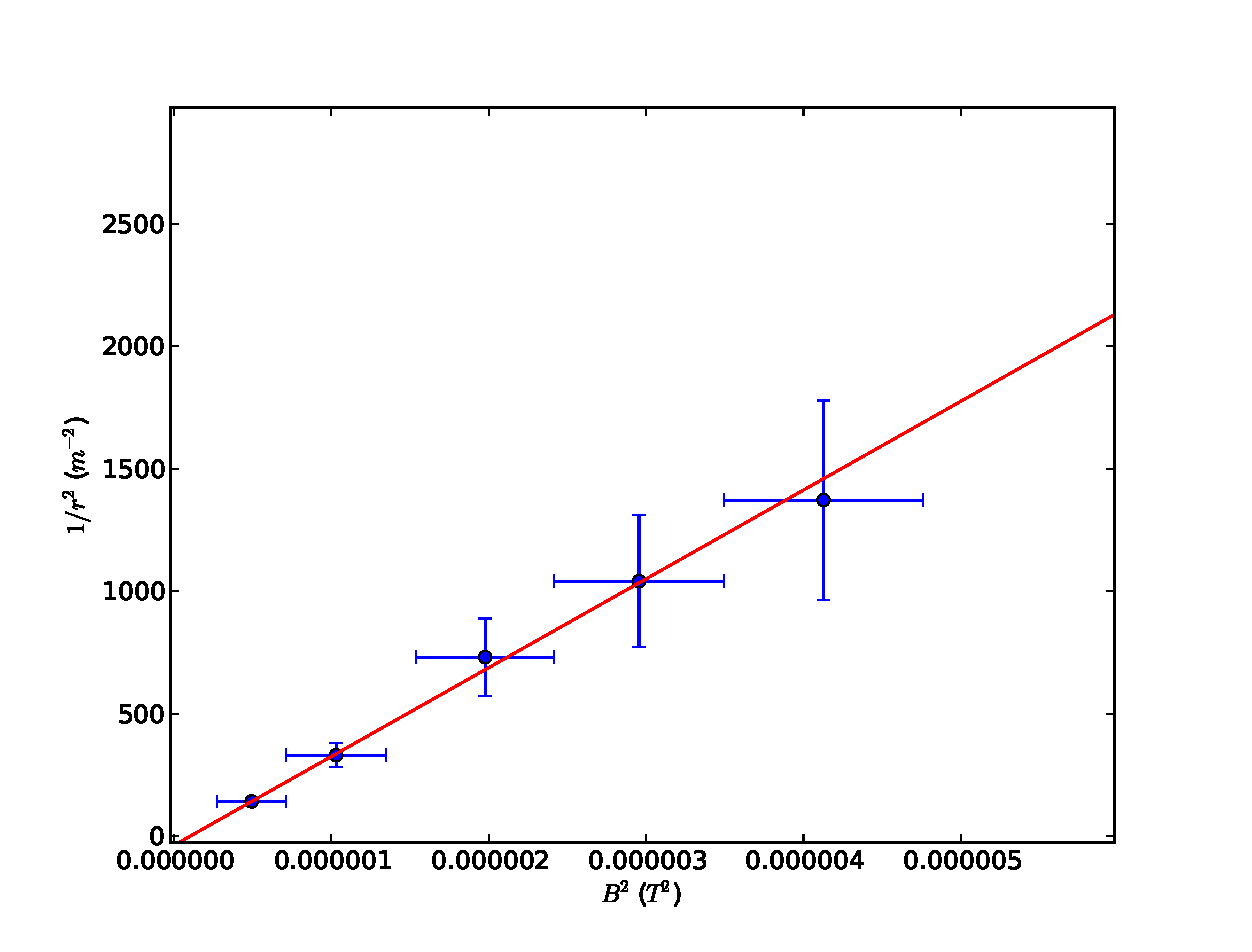
\includegraphics[width=0.5 \columnwidth]{fixedv.eps}
\end{figure}






\section{Results}

By using two error propagations, we will obtain two proper $\frac{e}{m}$ ratio:

\begin{table}[htdp]
\caption{ Experimental Data for voltage $V$ at ($250V$)}
\label{rawdata}
\centering
\begin{tabular}{ccc}
\\
Current ($A$)  & $r$ (cm)  \\
\hline
0.9 &  8.2   \\
1.3 &  5.3   \\
1.8 &  3.5   \\
2.2 &  3.3   \\
2.6 &  2.9   
\end{tabular}
\label{default}
\end{table}%

\begin{table}[htdp]
\caption{Fixed Current }
\label{rawdata}
\centering
\begin{tabular}{cccccc}
\\
$\frac{e}{m}$   & $\sigma_{\frac{e}{m}}$ & $m$ & $\sigma_{m}$ & $B$ & $\sigma_{B}$  \\
\hline
$1.79x{10}^{11}$  & $3.90x{10}^{10}$ & $5.46x{10}^{4}$ & $3.87x{10}^{3}$ & $7.81x{10}^{-4}$ & $7.81x{10}^{-5}$
  
\end{tabular}
\label{default}
\end{table}%

\begin{table}[htdp]
\caption{Fixed Voltage }
\label{rawdata}
\centering
\begin{tabular}{cccccc}
\\
$\frac{e}{m}$   & $\sigma_{\frac{e}{m}}$ & $m$ & $\sigma_{m}$ & $V$ & $\sigma_{V}$  \\
\hline
$1.81x{10}^{11}$  & $2.74x{10}^{10}$ & $3.62x{10}^{8}$ & $5.29x{10}^{7}$ & $250$ & $10$
  
\end{tabular}
\label{default}
\end{table}%





The real value of electron mass ratio is $1.76 x {10}^{11}$ C/kg\\

\begin{itemize}
\item Part I\\
$\frac{error}{sigma}=\frac{|(1.79-1.76) x {10}^{11}|}{3.60 x {10}^{10}}= 0.07 $\, true value is in 1$\sigma$ range.

\item Part II\\

$\frac{error}{sigma}=\frac{|(1.81-1.76) x {10}^{11}|}{2.74 x {10}^{10}}= 0.18 $\, true value is in 1$\sigma$ range.




\end{itemize} 


                         
When we think thoroughly what can cause the experiment to have error is fundamentally instrumental errors (especially Voltmeter) and we were given. 




\begin{acknowledgements}
I would like to thank (Associate Professor) V.Erkcan Ozcan  and my partner Kadir Simsek for their contributions, and also to the teaching assistant Serhat Istin for his guidance during this experiment.

\end{acknowledgements}

\section{References}
\begin{itemize}
\item 	E. Gulmez, ”Advanced Physics Experiment”, Istanbul, Bogazici University Publication, 1999
\end{itemize}

\section{Appendix}

Python code for part I:
\begin{lstlisting}


from pylab import *


radius = array([ 3.9, 4.6, 5.2, 6.1, 6.9 ]) *1e-2		
sigma_radius = 0.004                                            

Voltage = array([ 110, 150, 170, 230, 290 ]) 			
sigma_Voltage = 10                                              




std_radius = 2*radius*sigma_radius
std_Voltage = ones(len(Voltage))*sigma_Voltage


radius=radius**2



x = radius
sx = std_radius
y = Voltage
sy = std_Voltage



S   = sum(1 / sy**2)
Sx  = sum(x / sy**2)
Sy  = sum(y / sy**2)
Sxx = sum(x**2 / sy**2)
Sxy = sum(x*y / sy**2)

delta = S*Sxx - Sx**2

n = (Sxx*Sy - Sx*Sxy) / delta
m = (S*Sxy - Sx*Sy) / delta

sn = sqrt(Sxx / delta)
sm = sqrt(S / delta)



errorbar(x,y,xerr=sx,yerr=sy,fmt='o')

xx = arange(0,6e-3,1e-5)
yy = n + m*xx

plot(xx, yy, 'r-')

xlabel('$r^{2}$ ($m^{2}$)',fontname='Ubuntu')
ylabel('$Voltage$ ($V$)',fontname='Ubuntu')


show()

print m
print sm

b=7.81e-4
sb=7.81e-5

print 2*m/(b)**2
print sqrt((4/(b**4))*((sm)**2) +  (16* (m**2) /(b**6))*((sb)**2)   )




\end{lstlisting}

Python code for part II:

\begin{lstlisting}

from pylab import *


radius = array([ 8.4, 5.5, 3.7, 3.1, 2.7 ])*1e-2 		
sigma_radius = 0.004                                      

current = array([ 0.9, 1.3, 1.8, 2.2, 2.6 ]) 				
sigma_Current = 0.1 										
M_field = current*((8*1.26*1e-6*130)/(sqrt(125)*(0.15))) 	
sigma_M_field = sigma_Current*((8*1.26*1e-6*130)/(sqrt(125)*(0.15)))		

std_radius = 2*sigma_radius/radius**3
std_M_field = 2*sigma_M_field*2*M_field


radius=1/(radius**2)
M_field=M_field**2



y = radius
sy = std_radius
x = M_field
sx = std_M_field



S   = sum(1 / sy**2)
Sx  = sum(x / sy**2)
Sy  = sum(y / sy**2)
Sxx = sum(x**2 / sy**2)
Sxy = sum(x*y / sy**2)

delta = S*Sxx - Sx**2

n = (Sxx*Sy - Sx*Sxy) / delta
m = (S*Sxy - Sx*Sy) / delta

sn = sqrt(Sxx / delta)
sm = sqrt(S / delta)

errorbar(x,y,xerr=sx,yerr=sy,fmt='o')

xx = arange(0,6e-6,1e-7)
yy = n + m*xx

plot(xx, yy, 'r-')

xlabel('$B^{2}$ ($T^{2}$)',fontname='Ubuntu')
ylabel('$1/r^{2}$ ($m^{-2}$)',fontname='Ubuntu')


show()

print m
print sm

V=250
sv=10

print 2*m*V
print sqrt(4*V**2*sm**2+4*m**2*sv**2)



\end{lstlisting}

\end{document}
